\chapter{Introduction}
Abstract algebra, the study of algebraic structures is comparatively a new branch in mathematics that is being explored by many mathematicians. In recent years, applications of algebraic structures are explored in many fields. As an example, similar to differential equations on a function space, a time dependent partial differential equation can be studied using semigroup \cite{liaqat2021some}. Kleene algebra, semigroup structures are used in finite automata to better model and understand the finite state machines. Groups are one of the oldest structures that are used in number theory, in atomic and molecular theory, cryptography \cite{enwiki:1133598242}. Quasigroups and loops are used in encryption techniques for image data \cite{didurik2018some}. The simplest algebraic structure is magma. A magma has a set with a binary operation that is closed by definition. A magma with associative property is called a semigroup and with division operation is called a quasigroup. Figure ~\ref{fig_magma} shows the algebra hierarchy from magma to group. 
 \begin{figure}[ht]
	\centering
	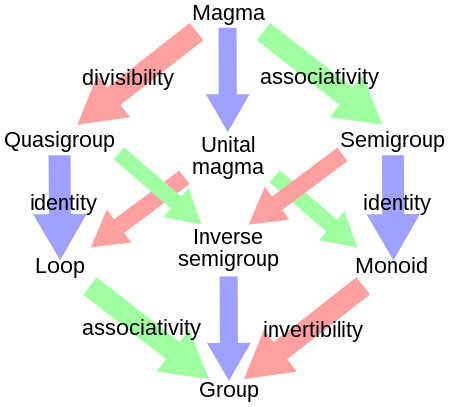
\includegraphics[width=0.7\textwidth]{figures/Sample/Magma_to_group.jpg}
	\caption{Algebraic structure hierarchy \cite{enwiki:1107380309}}
	\label{fig_magma}
\end{figure}
\\

With growing help of technology, mathematicians are more indulged in automated reasoning. Increasing powers of computers, software tools that help towards automated reasoning becomes useful in their research. Although the proof systems that support first order logic are successful, developing a tool that supports higher order logic is complex \cite{phillips2010automated}. Proof assistant systems are the bridge between computer intelligence and human effort. Agda, Coq, Isabelle, Lean and Idris are some of the commonly used proof assistant systems. These systems help in automated reasoning in deriving mathematical proofs. For the scope of the thesis we only discuss about algebraic structures in proof systems.\\


\section{Research Outline}
For any software system to be robust, the libraries of these systems should be strong. In the sense that the software tool should support the user with all necessary functionalities. There are some experiments on how to automate the process of generating libraries with minimum human effort \cite{BuildingDiamond}. These methods work in theory but becomes difficult in practice. For the complications in generated libraries, the standard libraries of proof systems do not rely on these generated code. This led to the question of what is the current scope of algebraic structures in the proof assistant systems. A survey was conducted to better understand the coverage of algebra in four proof systems agda, idris, lean and coq. Agda was one such system where there was better scope to contribute to the standard library. I was exposed to agda in course work as part of the program and added weight to chose agda over other systems. \\

As part of this thesis, more than twenty three structures was defined in the standard library for agda. Inspired by the application of structure semigroup, quasigroup, loop, ring, and kleene algebra, we define morphisms, direct product construct and prove some of the properties of the structures. One advantage of contributing to standard library is that others can use it to build on it.\\

When defining these structures, we analyze five problems that arise in programming algebra. Ambiguity in naming that is a structure can be misunderstood for other due to different usage of names in literature. Two structures that are equivalent but can be structurally different. When following the algebra hierarchy, it is possible to introduce redundant fields. A structure can be identical in the sense that it can have many names. Same structure can be expressed and defined in more than one way but they result in equivalent structures. To overcome these problems we briefly introduce the use of product family algebra.\\

\section{Thesis Outline}
We start with background knowledge on universal algebra in chapter 2. Chapter 3 gives a brief overview of agda in relevance with algebraic structures. Chapter 4 justifies the scope of the thesis contribution by a survey on algebraic coverage in proof systems. The next three chapters are dedicated to discuss the structures in details. Chapter 5 discuss the properties of semigroup and rings with variations of ring structure. Chapter 6 is dedicated to quasigroup and loop that uses division operation. Chapter 7 discuss about kleene algebra, definition, construct and properties. Chapter 8 describes the problems that should be handled when programming algebra in proof systems with a brief overview of product family algebra. Conclusion and future works are discussed in chapter 9.
